\chapter{檢視體資料}\label{ch:volume}
\index{Tishuju@體資料}

\chapterlead{原子結構告訴我們原子位於何處，體資料則描述空間中的數值如何變化。電荷密度、磁化密度以及其他標量場，都可以用等值面、切面或直接體渲染觀察。本章以 CHGCAR、Cube 和 XSF 為例，介紹如何選擇通道、讀懂單位、比較圖形，並匯出適合報告與進一步分析的結果。}

\section{讀懂體資料}
\index{Dianhe midu@電荷密度}
\index{Tishuju tongdao@體資料通道}

\subsection{體資料表示什麼}

一個三維標量場可以理解為空間網格上的一組數值。每個網格點具有位置和一個標量，檢視器用相鄰點之間的插值形成連續顯示。網格維度說明三個方向分別有多少取樣點；體素向量、原點和晶胞決定這些點在真實空間中的位置。

網格不一定與笛卡爾座標軸平行，也不一定正交。尤其在斜晶胞或來自其他程式的資料中，切片會隨網格取向而傾斜。觀察前先檢視檔案來源、維度和單位，再把圖形與原子結構聯絡起來。

同一個檔案可以含有多個通道。例如，自旋 CHGCAR 同時包含總電荷密度和磁化資訊；一個 Cube 檔案也可能存放多個資料集。切換通道改變的是正在顯示的標量場，而不只是配色。

\begin{table}[htbp]
\centering
\caption{常見體資料來源及其在檢視器中的解釋。}
\begin{tabularx}{\linewidth}{lX}
\toprule
檔案 & 主要內容與閱讀要點 \\
\midrule
CHGCAR、CHG & VASP 標量網格及原子結構。電荷密度按晶胞體積歸一化，使用 $\text{\AA}^{-3}$ 顯示；自旋檔案還有相關通道。\\
Cube、CUB & 原點、體素向量、原子以及一個或多個資料集。標量的物理意義取決於生成檔案的程式與任務。\\
XSF & 帶標籤的二維或三維 Datagrid，可帶原子結構。每個網格塊與其中的通道需按標籤辨認。\\
\bottomrule
\end{tabularx}
\end{table}

Cube 和 XSF 的標量不統一解釋為電子密度，介面可能顯示 \file{arbitrary}。這表示檢視器保留了源數值，而沒有為所有檔案強行指定同一個物理單位。即使圖形看起來像電荷分佈，也應依據計算來源解釋數值。

\subsection{\headinglatin{CHGCAR} 的自旋通道}
\index{CHGCAR@CHGCAR}

非自旋 CHGCAR 通常使用 \file{total}。對於共線自旋資料，\file{diff} 表示自旋差對應的磁化密度，檢視器還提供派生的 \file{up} 與 \file{down}：
\[
  \rho_{\uparrow}=\frac{\rho_{\mathrm{total}}+\rho_{\mathrm{diff}}}{2},
  \qquad
  \rho_{\downarrow}=\frac{\rho_{\mathrm{total}}-\rho_{\mathrm{diff}}}{2}.
\]
\file{diff} 中出現負值，並不表示總電子密度變成負數，而是說明所選自旋差的符號。非共線資料還可包含磁化的三個分量與模長，解釋時應區分分量的正負和向量模長。

\section{匯入體資料}

\begin{steps}
  \item 從側欄開啟\ui{專案瀏覽器}，雙擊頂層\ui{Volume}分類並選擇體資料檔案。示例可從 \file{CHGCAR.nospin.gz} 開始。若專案樹未顯示，在側欄面板庫的\ui{開啟面板}視窗選擇\ui{專案瀏覽器}。
  \item 等待初始檢視與摘要出現。先檢視檔名稱、\ui{Grid} 網格維度及 \ui{Units}，確認開啟了預期資料。
  \item 用左鍵拖動旋轉，滾輪縮放，右鍵拖動平移。按空格鍵居中並適配縮放。
  \item 在體資料檢視自己的工具欄開啟\ui{Viewer settings}，檢視當前 \ui{Channel} 與 \ui{Display mode}。先熟悉通道和模式，再修改外觀。
  \item 若檔案帶原子結構，保留晶胞與原子疊加，觀察標量場相對於原子的位置。
\end{steps}

較大資料可能先以較低顯示解析度出現，之後載入完整資料。狀態區域可顯示載入、構建或降級資訊。等待完成後再記錄網格或製作最終影象，避免把初始預覽誤作完整資料。

工具欄還提供自動旋轉、晶格軸與倒易軸方向、結構資訊、影象匯出、場景描述匯出和全屏。按 I 可隱藏或恢復摘要、分佈圖等輔助介面，使觀察區域更集中。需要記錄數值與單位時，則應把這些資訊重新開啟。

專案已有的體資料列在 \ui{Volume} 分類之下，雙擊具體條目即可重新開啟。頂層分類用於匯入新檔案，子條目用於檢視已匯入資料。側欄中的工作面板與體資料檢視內的顯示設定分別管理專案和影象，調整原子比例、通道或切面時使用檢視內的設定。

圖\ref{fig:volume-total-isosurface}顯示隨書非自旋檔案的總電荷密度等值面。淺藍色等值面與晶胞一起顯示，原子保留在場中，便於判斷分佈相對於結構的位置。檔案、通道與閾值的具體檢查見下一節。

\begin{figure}[H]
\centering
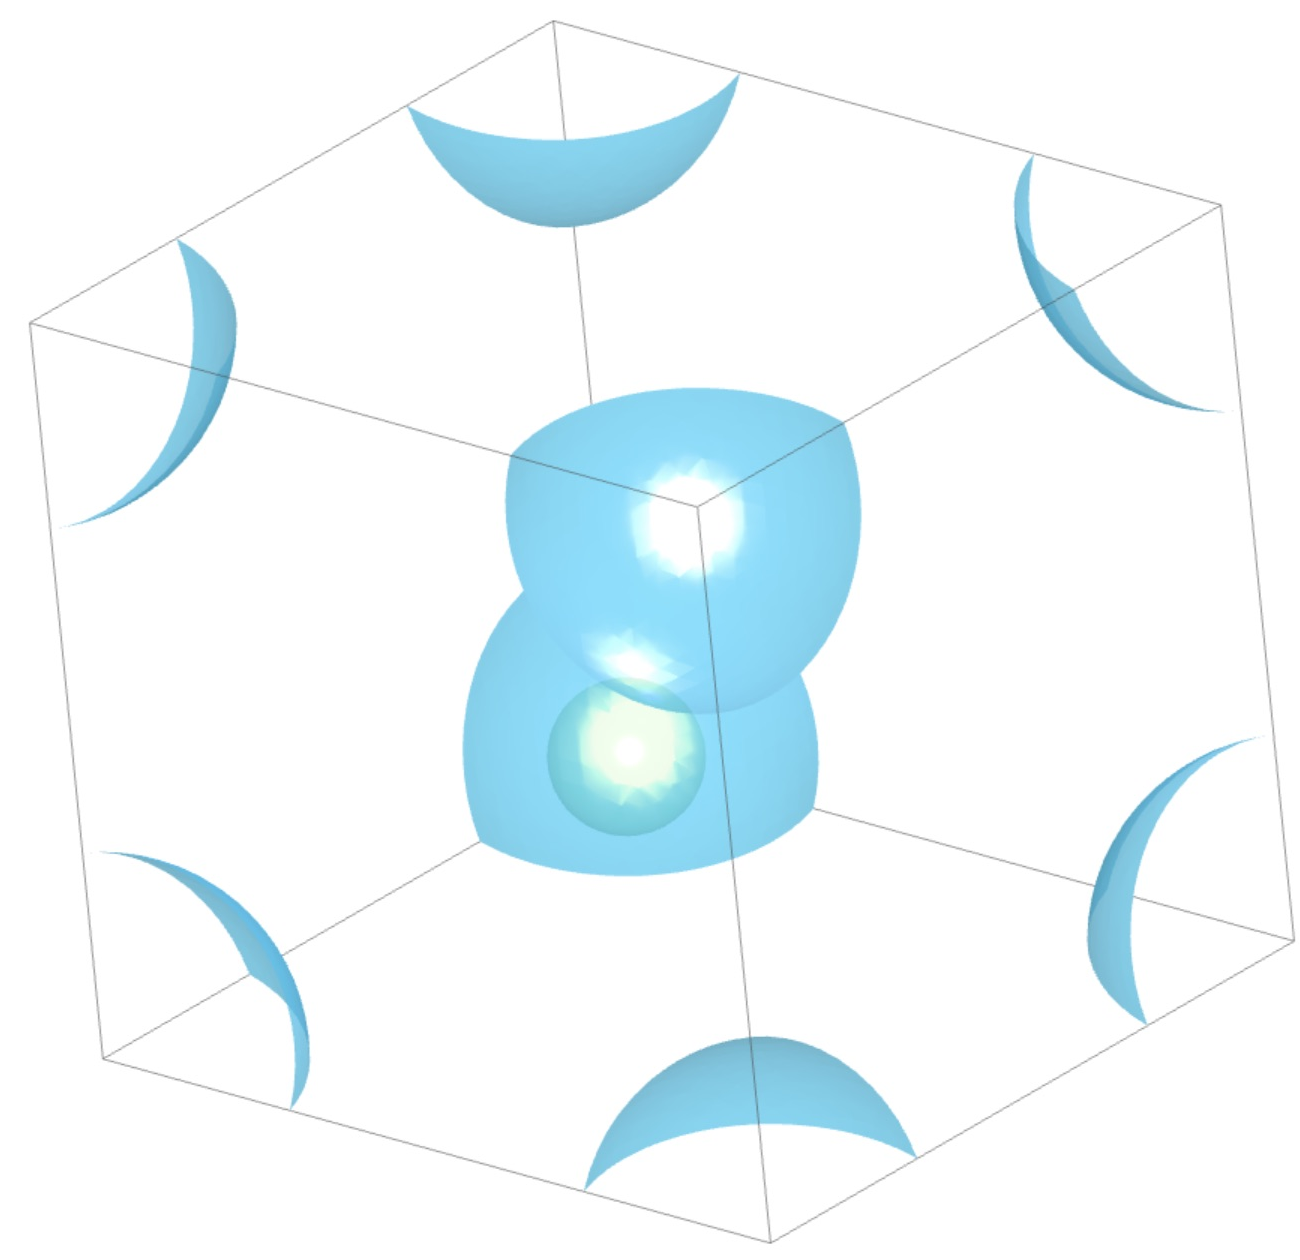
\includegraphics[width=112mm]{publication-assets/crop-53085697480f4dfda16f.png}
\caption{\file{CHGCAR.nospin.gz}的總電荷密度等值面。網格為$32\times32\times32$，通道為\ui{Total charge density}；正閾值為$0.04000\,\text{\AA}^{-3}$，負面關閉，透明度為0.72。}
\label{fig:volume-total-isosurface}
\end{figure}


\section{等值面：觀察同一數值形成的形狀}
\index{Dengzhimian@等值面}

\subsection{閾值決定看見什麼}

等值面連線標量值相同的位置。提高正閾值通常會使顯示集中到數值較高的區域，降低閾值則可能使面擴大或相互連通。沒有出現等值面時，先檢視閾值是否落在資料範圍內，以及該通道是否真的具有相應符號。


若以$s(\mathbf r)$表示當前通道的標量場，閾值為$\tau$，對應的等值面就是
\begin{equation}
  S_{\tau}=\{\,\mathbf r\mid s(\mathbf r)=\tau\,\}.
  \label{eq:volume-isosurface}
\end{equation}
它固定的是數值，表面的位置和形狀由資料決定。切面則先固定一個空間平面，再用顏色表示平面上各點的$s$值。二者所回答的問題不同，如圖\ref{fig:volume-surface-slice-concept}所示；直接體渲染又進一步沿視線組合一段體積中的資訊。

\begin{figure}[htbp]
\centering
\begin{tikzpicture}[x=1mm,y=1mm,font=\sffamily\small]
  \node[text=brand] at (25,45) {等值面：固定数值};
  \node[text=brand] at (89,45) {切面：固定位置};
  \foreach \dx in {0,64} {
    \draw[draw=muted!55,line width=.4pt]
      ({5+\dx},4) rectangle ({39+\dx},30);
    \draw[draw=muted!55,line width=.4pt]
      ({5+\dx},30) -- ({14+\dx},38) -- ({48+\dx},38)
      -- ({48+\dx},12) -- ({39+\dx},4);
    \draw[draw=muted!55,line width=.4pt] ({39+\dx},30) -- ({48+\dx},38);
    \draw[dashed,draw=muted!40,line width=.4pt]
      ({5+\dx},4) -- ({14+\dx},12) -- ({48+\dx},12);
    \draw[dashed,draw=muted!40,line width=.4pt]
      ({14+\dx},12) -- ({14+\dx},38);
  }
  \filldraw[fill=teal!25,draw=teal,line width=.7pt]
    (26,21) ellipse (13 and 10);
  \draw[draw=teal!65,dashed,line width=.5pt] (13,21) arc (180:0:13 and 3.2);
  \draw[draw=teal!65,line width=.5pt] (13,21) arc (180:360:13 and 3.2);
  \node[text=brand] at (26,25) {$s=\tau$};
  \filldraw[fill=paleblue,draw=brand,line width=.7pt]
    (69,17) -- (103,8) -- (112,25) -- (78,34) -- cycle;
  \begin{scope}
    \clip (69,17) -- (103,8) -- (112,25) -- (78,34) -- cycle;
    \fill[teal!25] (88,21) ellipse (14 and 11);
    \fill[teal!50] (88,21) ellipse (9 and 7);
    \fill[brand!65] (88,21) ellipse (4 and 3.2);
  \end{scope}
  \draw[draw=brand,line width=.7pt]
    (69,17) -- (103,8) -- (112,25) -- (78,34) -- cycle;
  \node[text=ink] at (25,-4) {形状随场与阈值改变};
  \node[text=ink] at (89,-4) {颜色表示平面上的场值};
\end{tikzpicture}
\caption{同一标量场的两种观察方式（概念示意）。等值面连接相同数值的位置；切面取一个平面，用色彩显示其内部变化。图中几何与色阶仅作概念示意。}
\label{fig:volume-surface-slice-concept}
\end{figure}


在\ui{Display mode} 中選擇 \ui{Isosurfaces}。正面與負面分別具有開關和閾值。總電荷密度通常主要觀察正面；磁化差、軌道等帶符號資料可能需要同時顯示兩種符號。透明度影響可見程度，不改變閾值和源資料。

\ui{Isovalue units} 提供三種閾值表示方式：絕對數值、標準差和百分位。絕對值適合明確的物理閾值；標準差按均值與分佈寬度描述位置；百分位則按資料分佈選擇閾值。比較兩個模型的絕對分佈時，應使用相同單位，並明確記錄各自閾值。


\ui{Absolute value}按所選顯示單位直接填寫$\tau$，並不把負值變成正值。選擇\ui{Standard deviations (σ)}時，輸入的是相對均值的標準差倍數$z$，實際閾值為
\begin{equation}
  \tau=\mu+z\sigma.
  \label{eq:volume-sigma-threshold}
\end{equation}
$\mu$和$\sigma$取自當前通道的網格數值，分別表示均值和標準差。$z=0$對應均值，$z=1$對應均值以上一個標準差，不能直接理解為場值等於1；若通道均值不為零，也不能把閾值簡寫成$z\sigma$。

\begin{table}[htbp]
\centering
\caption{閾值與顏色範圍中的量。}
\begin{tabularx}{\linewidth}{lX}
\toprule
量 & 介面中的意義\\
\midrule
$s$、$\tau$ & 當前通道值和等值面閾值；絕對輸入使用通道的顯示單位\\
$\mu$、$\sigma$ & 當前通道的均值和標準差；與通道值具有相同單位\\
$z$ & 標準差倍數，無量綱；用於將統計位置換成實際閾值\\
顏色上下限 & 指定色表覆蓋的數值區間，不改寫場值或CSV資料\\
\bottomrule
\end{tabularx}
\end{table}

\ui{Percentile}按網格樣本的數值排序選擇閾值。例如第90百分位描述該閾值在樣本分佈中的位置，並不表示等值麵包住了90\%的電子數或晶胞體積。切換通道後，均值、標準差和百分位都會隨資料改變，比較兩幅圖時要同時記錄閾值的表示方式。

\subsection{示例：檢視總電荷密度}

\begin{steps}
  \item 開啟\file{CHGCAR.nospin.gz}，核對摘要中的\ui{Grid}為$32\times32\times32$，\ui{Channel}為\ui{Total charge density}，單位為$\text{\AA}^{-3}$。
  \item 在顯示設定中選擇\ui{Isosurfaces}，將\ui{Isovalue units}設為\ui{Absolute value}。勾選\ui{Positive}，在其\ui{Threshold}中輸入\literalinput{0.04000}。
  \item 關閉\ui{Negative}，將\ui{Opacity}設為\literalinput{0.72}。這樣可以透過部分表面辨認內部原子，同時保留等值面的輪廓。
  \item 保留\ui{Atoms}和晶胞，暫時關閉\ui{Bonds}、\ui{Depth Cueing}、\ui{Boundary image atoms}與\ui{One-hop bonded atoms}，使畫面集中於場的分佈。
  \item 旋轉檢視，比較晶胞中部與邊界附近的等值面。記錄檔案、通道、單位、閾值與透明度，再匯出需要的影象。
\end{steps}

圖\ref{fig:volume-total-settings}把摘要與設定分別放大。先用左側確認讀入的資料，再用右側確認顯示條件，便不會把網格大小、密度閾值和透明度混為同一類引數。這裡的0.04000適用於本例檔案；換用其他資料時，應先檢視該通道的數值範圍，再選擇閾值。

\begin{figure}[H]
\centering
\begin{minipage}[t]{50mm}
\vspace{0pt}
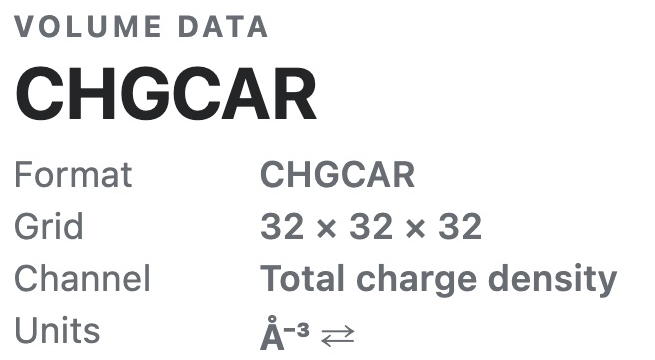
\includegraphics[width=\linewidth]{publication-assets/crop-817224ae41bbaff8bca4.png}
\end{minipage}\hfill
\begin{minipage}[t]{70mm}
\vspace{0pt}
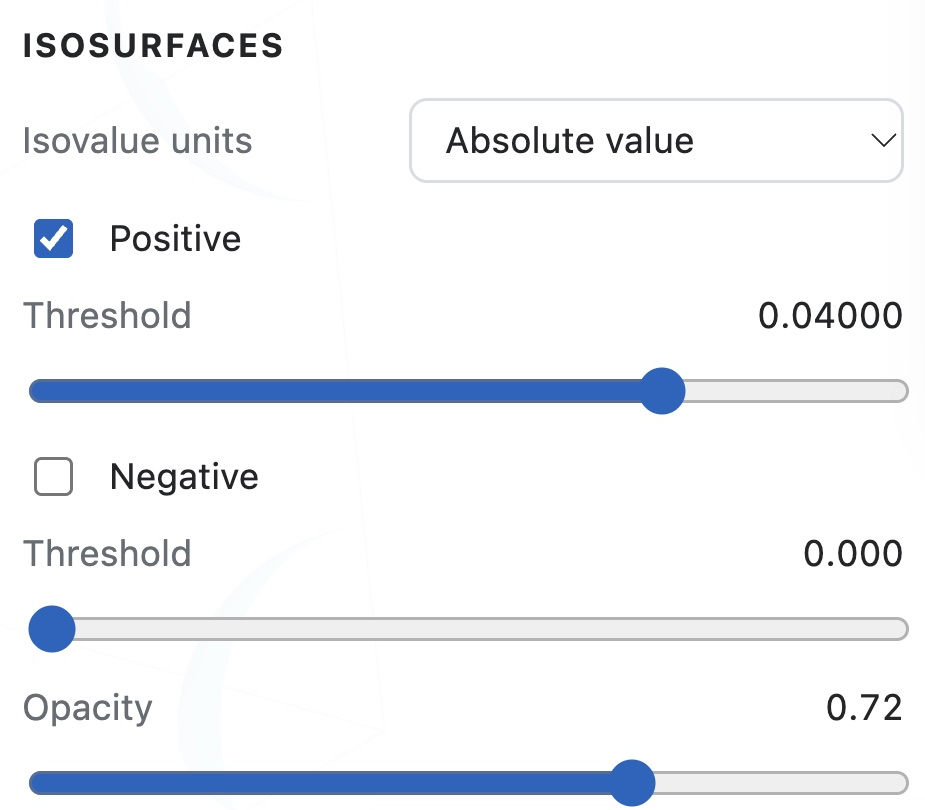
\includegraphics[width=\linewidth]{publication-assets/crop-f580c4c4a5007b46634f.png}
\end{minipage}
\caption{同一總密度檢視的摘要與閾值設定。左側列出網格、通道和單位；右側採用絕對閾值0.04000，關閉負面，透明度為0.72。}
\label{fig:volume-total-settings}
\end{figure}

\subsection{示例：比較自旋通道}

本例使用\file{CHGCAR.spin.gz}。開啟後先檢視總密度，再切到\ui{Magnetization density}，即\file{diff}通道。摘要中的網格變為$48\times48\times48$。當前通道在分佈圖中顯示的範圍約為$-0.001142$至$-0.0001356\,\text{\AA}^{-3}$，所有數值都在零以下。

\begin{steps}
  \item 在顯示設定中選擇\ui{Magnetization density}、\ui{Isosurfaces}和\ui{Absolute value}，核對摘要中的通道與單位。
  \item 勾選\ui{Negative}，在它下方的\ui{Threshold}輸入\literalinput{-0.0006000}。該值位於本例資料範圍內，應出現紅色負等值面。
  \item 將\ui{Opacity}設為\literalinput{0.72}，保留原子與晶胞，沿用前例關閉化學鍵及外圍映像的顯示設定。轉動檢視，觀察晶胞內部與邊界附近的表面。
  \item 可保持\ui{Positive}勾選、閾值為0，如圖\ref{fig:volume-diff-settings}。本檔案沒有零或正值，因此這個開關不會增加正等值面。圖中的綠色球體來自原子疊加，與等值面的正負開關分別控制。
  \item 繼續切換到\file{up}和\file{down}，檢視由總密度與差密度得到的兩個自旋通道。每次切換後重新檢查數值範圍與閾值，併為不同通道分別記錄顯示條件。
\end{steps}

負磁化密度表示當前自旋約定下的差密度為負，並不表示總電荷密度為負。本例說明負面開關與閾值的關係；若要同時觀察正、負兩種表面，需要所選資料本身具有相應的取值範圍。

\begin{figure}[H]
\centering
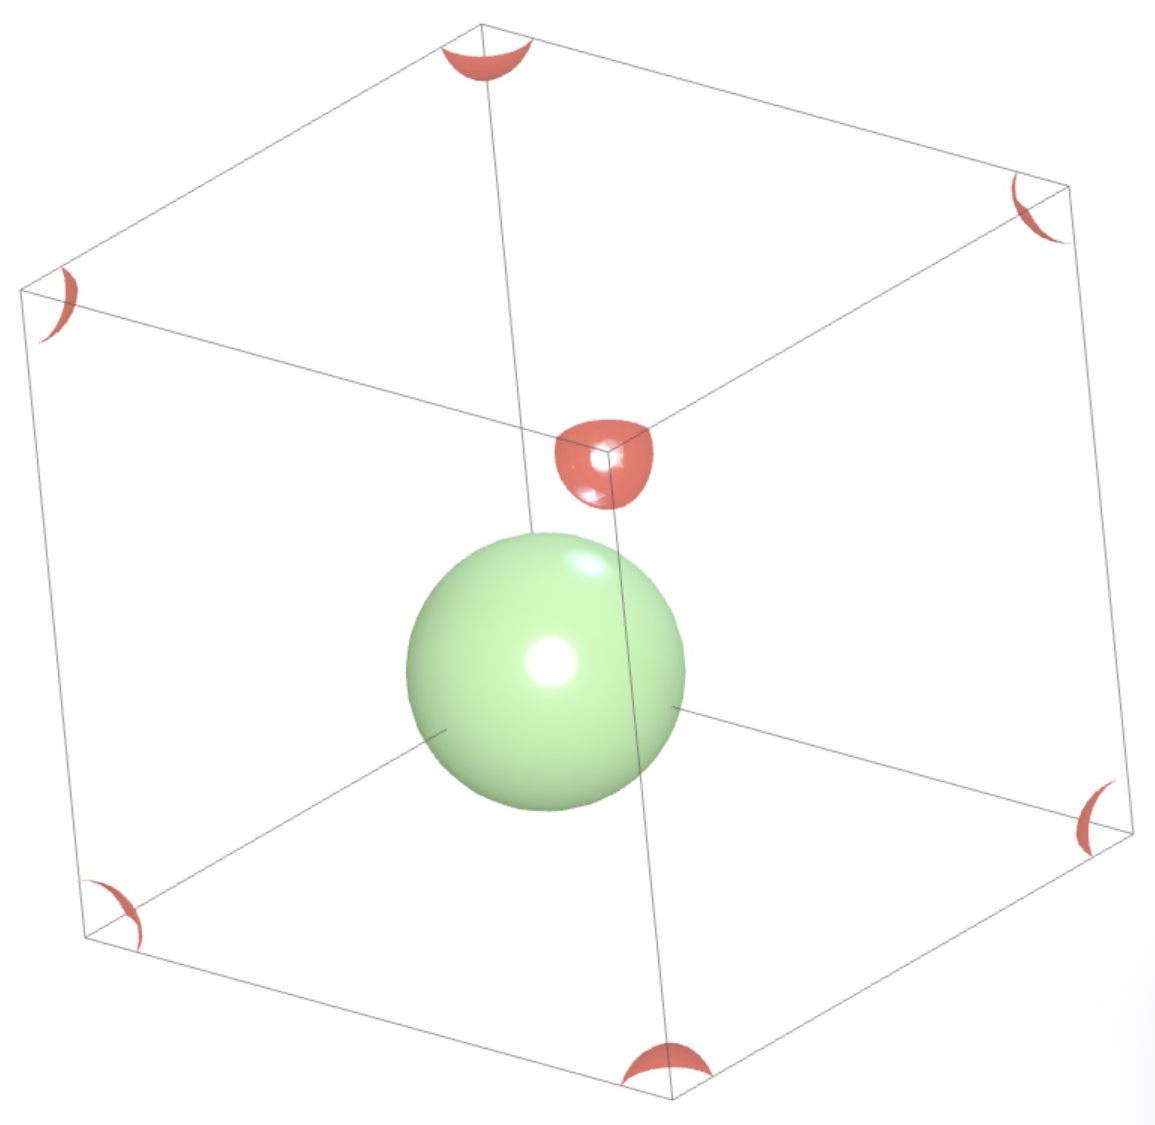
\includegraphics[width=112mm]{publication-assets/crop-eb58a23d11fe997c90a4.png}
\caption{\file{CHGCAR.spin.gz}中\ui{Magnetization density}通道的等值面。網格為$48\times48\times48$，紅色表面的閾值為$-0.0006000\,\text{\AA}^{-3}$，透明度為0.72；綠色球體是疊加顯示的原子。}
\label{fig:volume-diff-isosurface}
\end{figure}

\begin{figure}[H]
\centering
\begin{minipage}[t]{50mm}
\vspace{0pt}
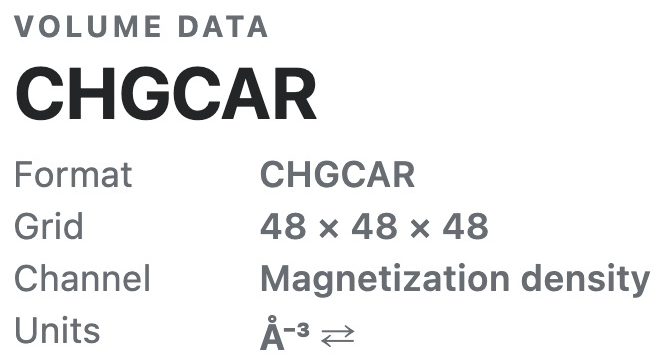
\includegraphics[width=\linewidth]{publication-assets/crop-1252e2f6c064962fc6d9.png}
\end{minipage}\hfill
\begin{minipage}[t]{70mm}
\vspace{0pt}
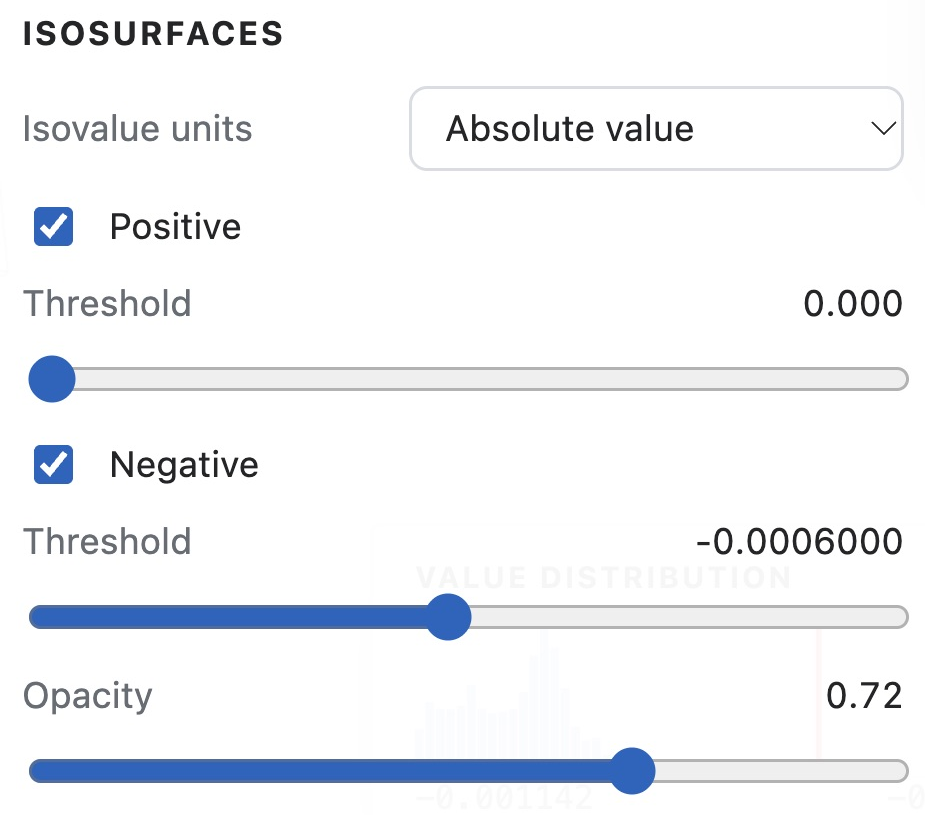
\includegraphics[width=\linewidth]{publication-assets/crop-6e54a4267b5bd8c4b3c0.png}
\end{minipage}
\caption{磁化密度的摘要與閾值設定。正面開關保留在0，負面閾值為$-0.0006000\,\text{\AA}^{-3}$。由於本通道全部為負，只形成負等值面。}
\label{fig:volume-diff-settings}
\end{figure}


\subsection{平滑與週期邊界}

\ui{Smooth vertex normals} 改善等值面的光照外觀，使三角面片之間的明暗更連續。它不會提高原始網格解析度。對於週期取樣資料，\ui{Wrap periodic boundaries} 可使邊界附近的等值面按週期關係連線；是否啟用應與檔案的週期性一致。

若邊界處出現表面截斷，先檢查晶胞邊界和週期設定，再判斷是否來自網格本身。使用較高質量的影象匯出可以使文字和邊緣更清楚，但無法彌補源資料取樣過粗的問題。

\section{\headinglatin{Miller} 切面：檢視內部數值}
\index{Qiemian@切面}
\index{Miller qiemian@Miller 切面}

\subsection{一個指陣列定義一個平面}

等值面適合看形狀，切面適合看一個截面內的連續變化。選擇 \ui{Miller plane slice} 後，設定中的 I、J、K 共同構成一組 Miller 指數，定義穿過體資料中心的單個平面。三項不能全為 0。

例如 $(0,0,1)$ 與 $(1,0,0)$ 選擇不同取向；$(1,1,0)$ 則可觀察斜截面。它們是同一個平面的方向引數，不是三張可以獨立移動的切片。在非正交網格中，切面按照實際體素向量確定空間方向，不能把 I、J、K 直接當作笛卡爾 $x$、$y$、$z$ 滑塊。


在三個方向均有多個取樣點的三維網格中，令$u,v,w$分別表示沿三個網格方向、從首個到末個取樣點的歸一化位置，範圍為0至1。介面中的I、J、K分別記為$h,k,l$，當前中心切面滿足
\begin{equation}
  h\left(u-\frac12\right)
  +k\left(v-\frac12\right)
  +l\left(w-\frac12\right)=0.
  \label{eq:volume-central-miller}
\end{equation}
$(0,0,1)$因此給出$w=1/2$；$(1,1,0)$給出$u+v=1$，仍經過網格中心。這裡的歸一化位置橫跨取樣範圍，不能一概當作完整晶胞的分數座標。檢視器再依據體素向量把該平面對映到真實空間，所以斜網格也保留相應取向。改變整陣列是在改變中心平面的方向，而不是沿某一軸移動它。

\subsection{示例：觀察 \headinglatin{Cube} 的(110)切面}

\begin{steps}
  \item 開啟\file{elec.cube.gz}，核對摘要中的網格為$23\times23\times24$，通道為\ui{Dataset 1}，單位為\file{arbitrary}。
  \item 在顯示設定中選擇\ui{Miller plane slice}，將 I、J、K 三個數值分別設為1、1、0。
  \item 在\ui{Colormap}中選擇\ui{Cool--warm}，將\ui{Interpolation}設為\ui{Linear}。\ui{Range minimum}保留\literalinput{0.0034185}，把\ui{Range maximum}改為\literalinput{0.2}。
  \item 保留原子與晶胞，將\ui{Atom scale}設為\literalinput{0.22}；關閉化學鍵、配位多面體、深度明暗及外圍映像，使傾斜平面更容易辨認。
  \item 關閉設定面板，轉動模型，觀察切面穿過晶胞的位置及原子相對於平面的分佈。需要比較取樣效果時，可切換\ui{Nearest}，觀察分塊，再恢復\ui{Linear}。
  \item 記錄切面指數、色表、顏色範圍和插值方式，再從\ui{Slice export}匯出PNG或CSV。匯出檔案的內容見本章後面的匯出小節。
\end{steps}

圖\ref{fig:volume-miller110}採用較低的顏色上限，使切面中數值較小區域的變化更明顯。超過0.2的值使用色表的高階顏色顯示，源資料仍保留原值；CSV也不會將它們截為0.2。本例的紅藍表示所選數值區間的兩端，不能僅憑顏色判斷數值的正負。

\begin{figure}[H]
\centering
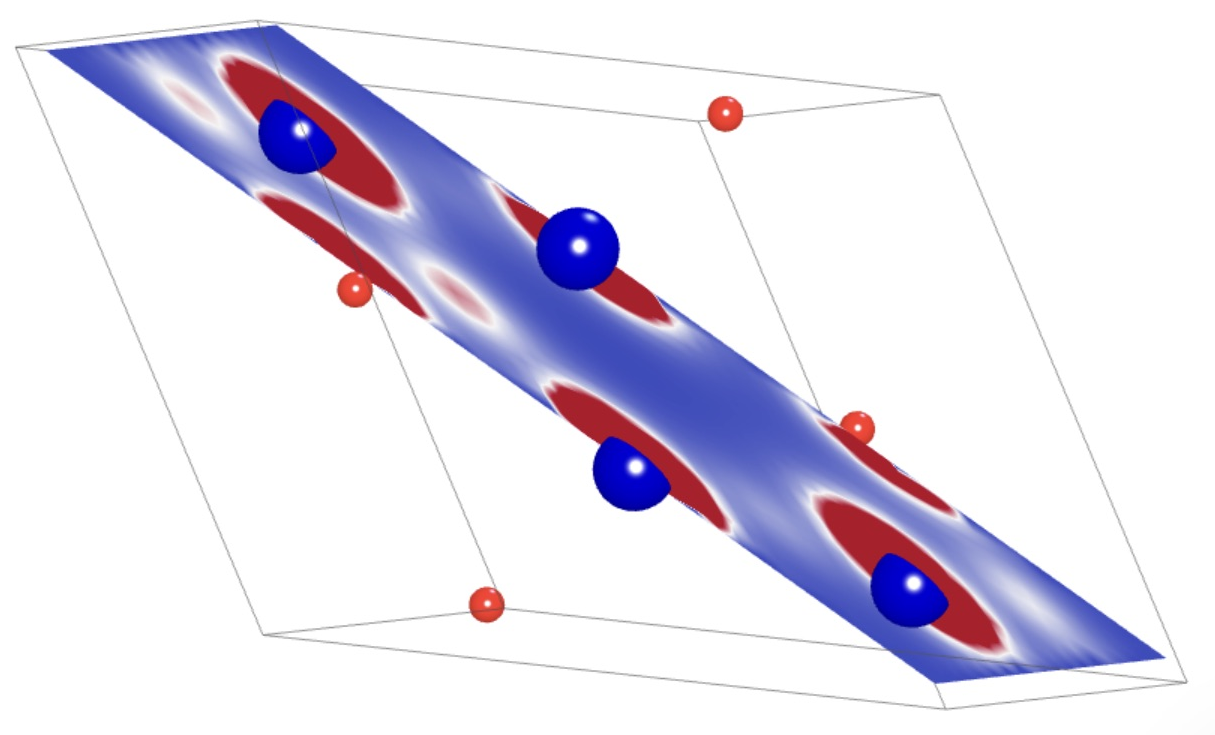
\includegraphics[width=112mm]{publication-assets/crop-aa00ad998951381ace74.png}
\caption{\file{elec.cube.gz}的(110)切面。網格為$23\times23\times24$，通道為\ui{Dataset 1}，標量單位為\file{arbitrary}；採用\ui{Cool--warm}、線性插值和0.0034185至0.2的顏色範圍。}
\label{fig:volume-miller110}
\end{figure}

\begin{figure}[H]
\centering
\begin{minipage}[t]{50mm}
\vspace{0pt}
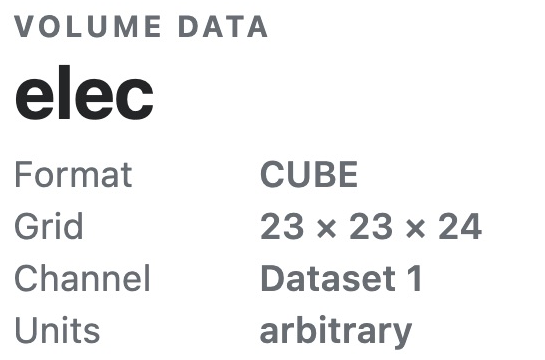
\includegraphics[width=\linewidth]{publication-assets/crop-ab9df592529bd047787b.png}
\end{minipage}\hfill
\begin{minipage}[t]{70mm}
\vspace{0pt}
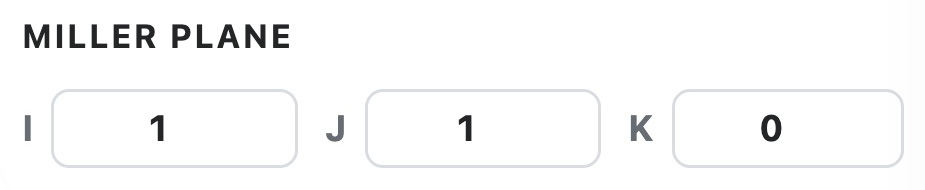
\includegraphics[width=\linewidth]{publication-assets/crop-1de9d3c6e62d7816cea2.png}
\par\vspace{2mm}
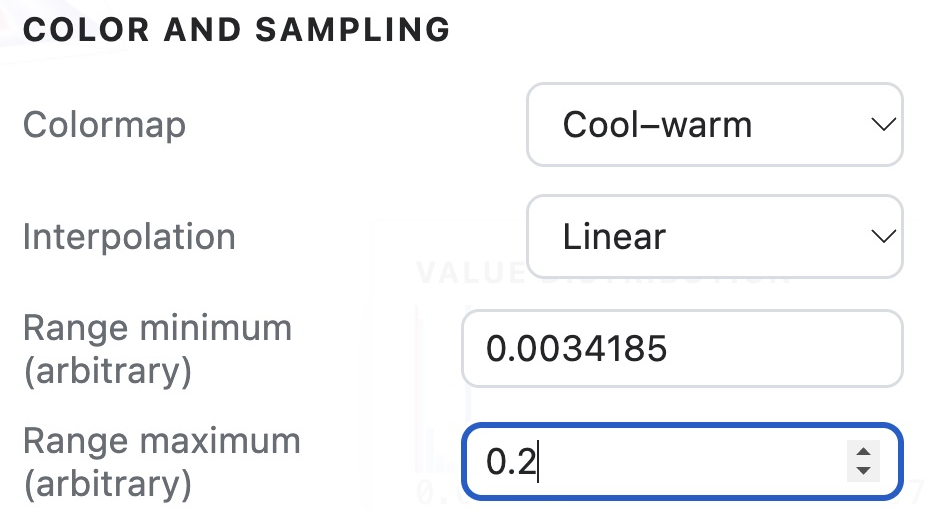
\includegraphics[width=\linewidth]{publication-assets/crop-209a06fc6024f4d5e0ba.png}
\end{minipage}
\caption{切面摘要和設定區域性。左側核對檔案、網格與單位；右側上方填寫同一組Miller指數，下方設定色表、插值及顏色範圍。顏色上限0.2只控制顯示。}
\label{fig:volume-miller110-settings}
\end{figure}

還可以開啟\file{datagrid_3d.xsf}，先按標籤辨認通道，再重複切面練習。比較兩個檔案時，既看網格的空間取向，也看標量本身的含義；相同的(110)指數並不要求兩張圖具有相同尺寸或數值範圍。


\subsection{顏色範圍與分佈圖}

\ui{Range minimum} 和 \ui{Range maximum} 決定哪些數值對映到色表兩端。範圍較寬時，區域性變化可能不明顯；適當縮小範圍可以突出感興趣的區間。超出顏色範圍的值仍然存在，只是採用端點顏色顯示。

\ui{Value Distribution} 展示當前通道的數值分佈。在等值面模式中，點選分佈圖可以設定相應正、負閾值；在切面或直接體渲染中，點選則調整較近的顏色範圍端點，也可拖動標記細調。它是選擇顯示區間的工具，不是能譜，也不是沿某條空間路徑的剖面。

對於帶正負的場，\ui{Cool--warm} 常便於辨認兩側；對於非負場，連續色表通常更容易閱讀。比較不同模型時應儘量保持同一色表與顏色範圍，使顏色差異具有相同含義。

\section{直接體渲染與結構疊加}
\index{Zhijie ti xuanran@直接體渲染}

直接體渲染沿視線累積標量場的顏色與透明度，可以同時看到較大範圍的內部變化。在\ui{Display mode} 中選擇 \ui{Direct volume (GPU)}，再按需要調整透明度、梯度透明度和取樣質量。\ui{Fast} 適合互動觀察，\ui{Balanced} 用於一般檢視，\ui{High} 適合在裝置允許時檢查細節。

I、J、K 的裁剪上下限以 0 到 1 的比例表示，可去掉盒子的一部分，使內部更易觀察。例如，將一個方向的範圍從 0--1 縮到 0.25--0.75，可以聚焦中部區域。裁剪改變顯示範圍，不會刪除檔案中的資料。

\subsection{示例：沿網格方向檢視中部體積}

繼續使用前例的\file{elec.cube.gz}，便於比較同一份資料在切面和體渲染中的不同表現。切面顯示一個平面上的數值，體渲染則沿視線疊加一段體積中的顏色與透明度，因此兩種模式的明暗不必逐點相同。

\begin{steps}
  \item 核對檔案仍為\file{elec.cube.gz}，通道為\ui{Dataset 1}，網格為$23\times23\times24$，單位為\file{arbitrary}。將\ui{Display mode}切換為\ui{Direct volume (GPU)}。
  \item 沿用\ui{Cool--warm}、\ui{Linear}及0.0034185至0.2的顏色範圍。先保持顏色設定一致，再比較顯示方式。
  \item 將\ui{Sampling quality}設為\ui{Balanced}，\ui{Opacity}設為\literalinput{0.72}，\ui{Gradient opacity}設為\literalinput{0.35}。後者調整區域性變化對透明度的影響，可與整體透明度分別試調。
  \item 將\ui{I clipping}的下限與上限分別設為\literalinput{0.25}、\literalinput{0.75}；\ui{J clipping}與\ui{K clipping}均保留0和1。此時只顯示I方向中間一半的體積，另外兩個網格方向保持完整。
  \item 保留原子與晶胞，關閉化學鍵、多面體及外圍映像。關閉設定面板並按I隱藏摘要與分佈圖，轉動檢視觀察內部的連續變化。需要核對檔案資訊時，再按I恢復輔助介面。
\end{steps}

圖\ref{fig:volume-direct}展示直接體渲染效果，設定區域性見圖\ref{fig:volume-direct-settings}。I、J、K在這裡表示網格方向上的裁剪比例，與前節Miller切面的整陣列定義不同；它們也不一定與全域性笛卡爾座標軸重合。將裁剪恢復為0至1即可重新顯示完整體積，源網格仍為$23\times23\times24$。

\begin{figure}[H]
\centering
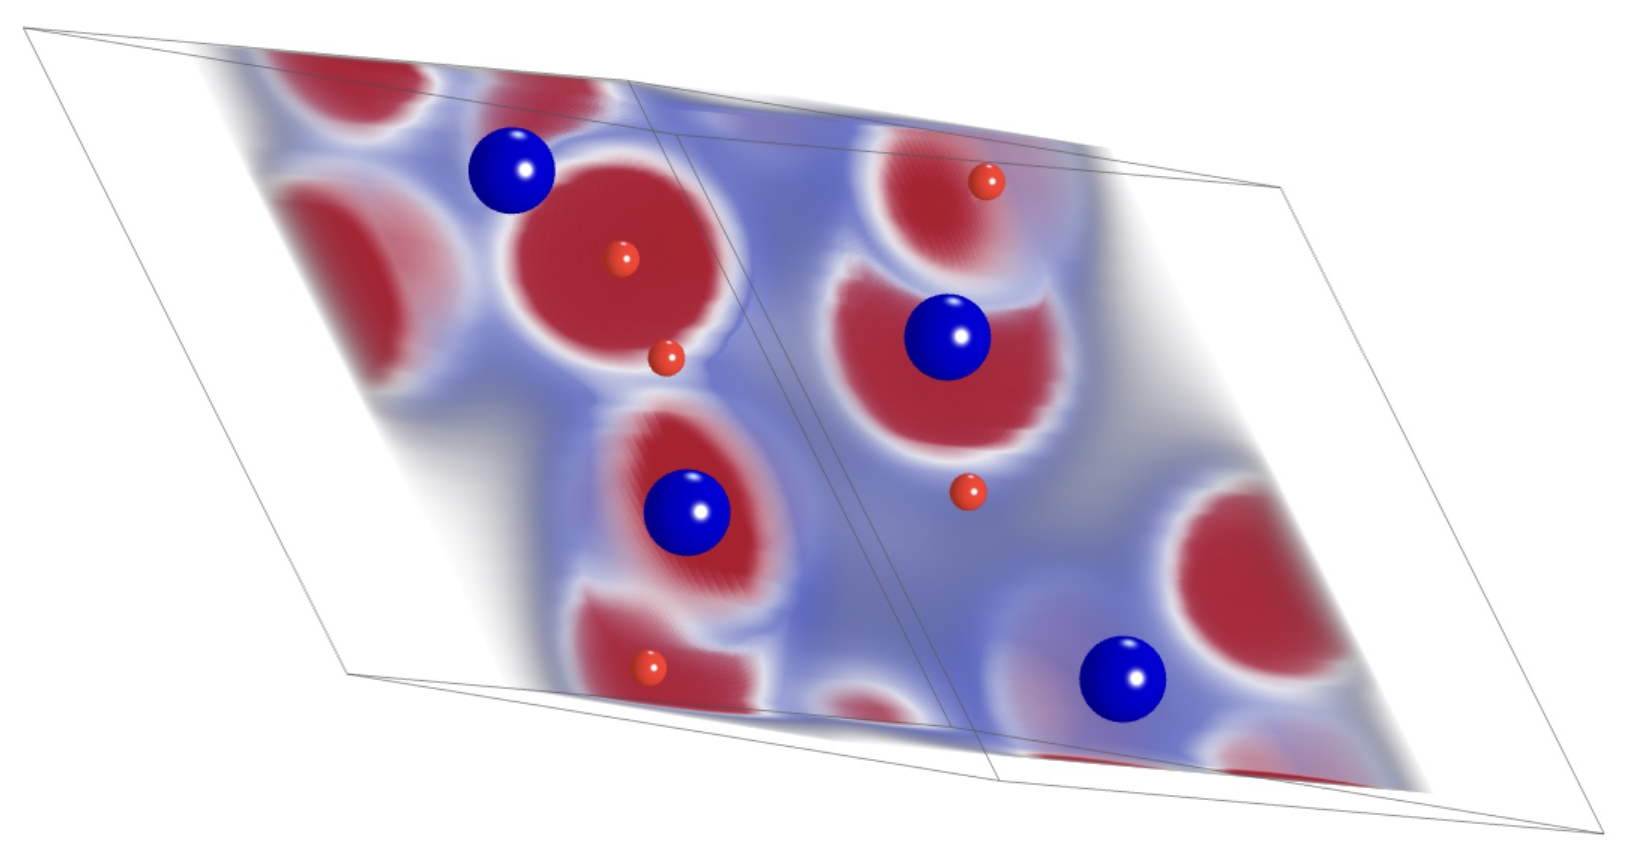
\includegraphics[width=112mm]{publication-assets/crop-68bb0517e51ea1057170.png}
\caption{\file{elec.cube.gz}的直接體渲染畫面。顯示模式為\ui{Direct volume (GPU)}；\ui{Dataset 1}的顏色範圍為0.0034185至0.2，I方向顯示0.25至0.75，原子與完整晶胞輪廓用於定位。}
\label{fig:volume-direct}
\end{figure}

\begin{figure}[H]
\centering
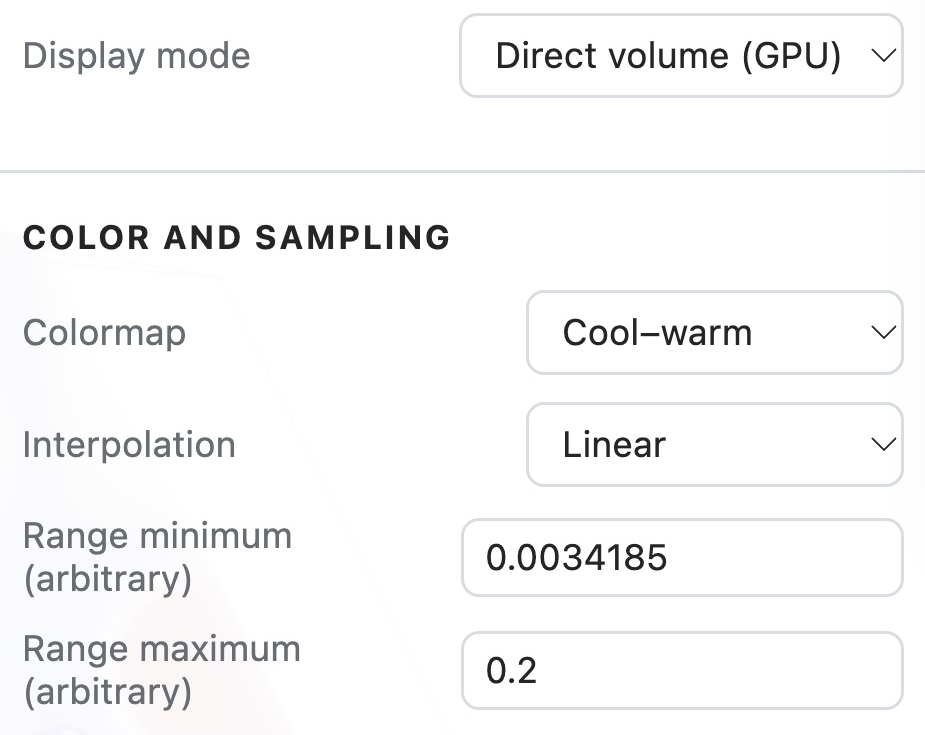
\includegraphics[width=80mm]{publication-assets/crop-3b2d9027085c84d05818.png}
\par\vspace{2mm}
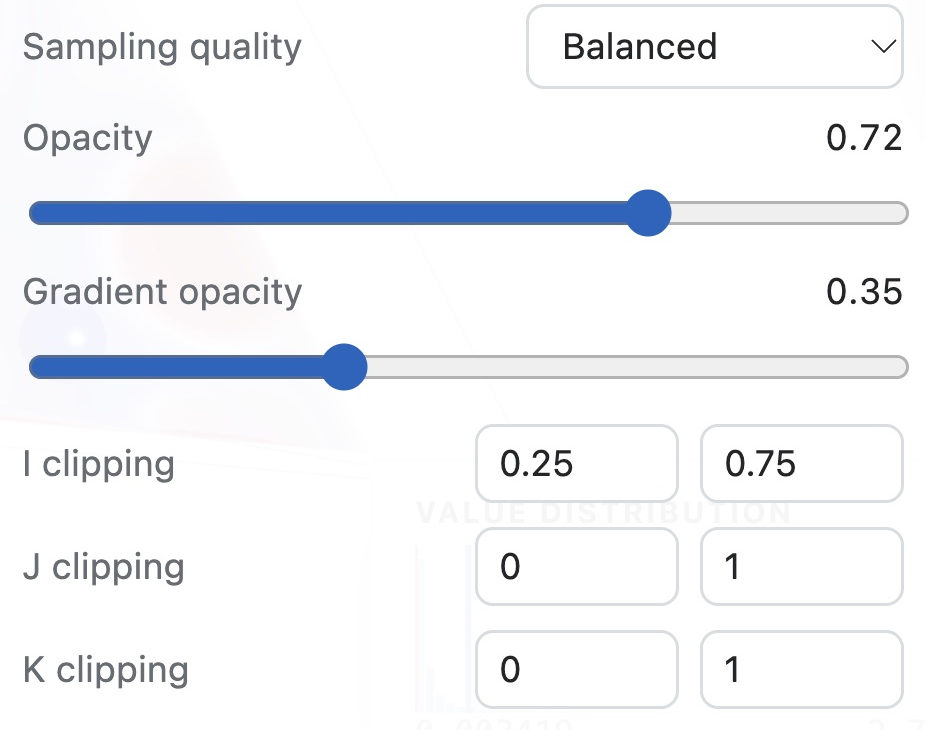
\includegraphics[width=80mm]{publication-assets/crop-7567d94dfd7d877833b9.png}
\caption{直接體渲染設定。上方為模式、色表、插值和顏色範圍；下方為\ui{Balanced}取樣質量、0.72透明度、0.35梯度透明度及三個方向的裁剪比例。}
\label{fig:volume-direct-settings}
\end{figure}

\subsection{用結構疊加定位場}

若體資料包含原子結構，\ui{Visibility} 中可以控制原子、化學鍵、晶胞、配位多面體、方向軸、週期邊界原子及磁矩等物件。先保留用於定位的少量物件，再逐一增加輔助顯示，通常更容易看清場與結構的關係。

\ui{Lighting \& surface} 控制原子疊加的環境光、方向光、金屬度、粗糙度、亮度和對比度。它們影響影象外觀，不改變標量場的大小。製作一組比較圖時，保持這些設定一致，並把決定科學含義的通道、閾值和單位寫入圖注。


\section{匯出體資料}
\index{Daochu tuxiang yu shuju@匯出影象與資料}

\subsection{在檢視中取樣}
\index{Caiyang@取樣數值}

雙擊體資料可以顯示取樣值與網格位置。點探針使用三線性插值，數值不一定等於某一個原始網格點。需要精確比較時，應記錄通道與取樣位置，並使用取樣數值。切面中的最近鄰或線性選項另用於切面顯示與匯出，不改變點探針的插值方式。

選擇疊加原子時，體資料檢視內的原子資訊區域可顯示笛卡爾與分數座標，複製按鈕保留比面板簡寫更多的數值精度。原子座標與標量取樣是不同的資訊：一個用於定位原子，一個用於讀取空間場。

對於可轉換的密度單位，\ui{Density units} 可在 $\text{\AA}^{-3}$ 與 $\mathrm{bohr}^{-3}$ 之間切換。切換單位會改變顯示數值，所代表的物理密度保持相同。比較圖表和報告時，統一單位後再比較數值。

\subsection{匯出當前影象}

影象匯出選單提供 PNG、JPEG、TIFF、SVG，以及向量和柵格兩類 PDF。PNG 和 TIFF 適合保留清晰的柵格圖；JPEG 便於壓縮分享；SVG 和 PDF 適合插入排版流程。匯出前先停止自動旋轉，選定取景，確認希望保留的原子、晶胞和輔助物件。

匯出影象時，在正文或圖注寫明檔案來源、通道、閾值或顏色範圍、單位與必要取向，並保留相應原始資料。

\subsection{匯出等值面和切面}
\index{CSV@CSV 匯出}

在等值面模式下，\ui{Isosurface export} 提供 glTF、GLB、PLY 和 STL，用於把當前等值面幾何送入其他三維工具。不同格式儲存的資訊不完全相同；使用外部軟體後應核對尺寸和外觀，座標按 \AA 理解。

在切面模式下，\ui{Slice export} 提供 PNG 和 CSV。切面 PNG 用於儲存當前平面的顏色圖；CSV 用於後續作圖或數值分析。CSV 先列出網格位置 \file{i}、\file{j}、\file{k}，再列出以 \AA 為單位的笛卡爾位置 \mbox{\file{x_angstrom}}、\mbox{\file{y_angstrom}}、\mbox{\file{z_angstrom}}，最後是當前通道的源數值 \file{value}。切面邊界外的取樣位置可能沒有有效值，分析時應按資料有效範圍處理。

匯出後可以做一次簡單核對：重新開啟 PNG，確認取向、色表和感興趣區域；再檢視 CSV 表頭，確認座標單位與數值列。若希望把兩套模型的同一切面畫在同一張圖中，應先保證切面的空間定義、網格範圍和通道一致。相同的 Miller 指數給出相同型別的方向，但晶胞改變後，平面的真實尺寸和經過的位置仍可能不同。

本例匯出檔案為\file{elec.total.slice-1_1_0.csv}與同名PNG。CSV有1568個取樣位置，其中778個具有有限數值，另790個在體資料邊界外，\file{value}記為\file{NaN}。NaN不表示數值為零，作圖或統計時應先篩選有效值。

這些有效切面值約為0.003525至2.3995，其中147個仍大於顯示上限0.2，可以用來核對顏色設定與源數值的區別。切面PNG為$384\times768$畫素，顯示取樣平面中的顏色分佈；圖\ref{fig:volume-miller110}同時呈現切面在晶胞中的取向。

\Needspace{8\baselineskip}
\begin{notebox}{顯示單位與 CSV}
CSV 的座標列以 \AA 輸出，數值列保留通道內部採用的單位。對於 \mbox{CHGCAR}，密度數值按 $\text{\AA}^{-3}$ 理解；介面切換為 $\mathrm{bohr}^{-3}$ 時，CSV 數值列仍使用 $\text{\AA}^{-3}$。Cube 和 XSF 的標量單位則應按原始檔說明記錄。
\end{notebox}

\ui{Export scene JSON} 匯出場景描述，便於保留網格、通道及結構等說明資訊。它不包含完整體素陣列，也不能代替儲存原始場檔案；相機位置和臨時顯示設定需另行記錄。需要重現影象時，另記閾值、顏色範圍和取景，並同時保留原始資料。

\subsection{組織一組可比較的結果}

完成一次觀察後，可以為資料與影象建立對應名稱，例如在檔名中包含體系、通道和切面。對 CHGCAR 的 \file{total} 與 \file{diff} 分別保留影象，避免用“密度圖”概括含義不同的通道。在圖注中說明正負面的顏色和閾值；在切面圖中說明顏色範圍。讀者無需開啟原檔案，也應能判斷圖上顏色和表面代表什麼。

若圖形用於研究報告，可保留一張帶完整摘要和設定的工作截圖，再匯出一張佈局整潔的結果圖。前者便於自己複查，後者用於正文展示。最終選擇應圍繞要說明的現象：等值面強調形狀和連線，切面強調區域性變化，體渲染強調空間層次，三者各有用處。

\section{影象沒有按預期出現時}

等值面為空，先檢查通道、正負面開關和閾值範圍。切面顏色幾乎一致，檢視顏色範圍是否過寬。原子遮擋場，減小原子比例或暫時隱藏化學鍵和多面體。旋轉後找不到模型，按空格鍵重新居中。

直接體渲染需要相應的圖形支援。若裝置不能使用 WebGL2，檢視器可採用 CPU 切片方式，並繼續提供切片 PNG/CSV 匯出；三維紋理容量不足時也可能回到切面。介面顯示的降級原因有助於選擇當前裝置可用的模式。二維XSF使用切面顯示。

最後，插值、平滑和更大的匯出圖片都只改善顯示。若研究問題需要更細的空間資訊，應回到計算階段提高源網格解析度，再重新檢查收斂。這樣，影象中的細節才有相應資料作為依據。
